%% start of file `template.tex'.
%% Copyright 2006-2013 Xavier Danaux (xdanaux@gmail.com).
%
% This work may be distributed and/or modified under the
% conditions of the LaTeX Project Public License version 1.3c,
% available at http://www.latex-project.org/lppl/.


\documentclass[11pt,a4paper,roman]{moderncv}        % possible options include font size ('10pt', '11pt' and '12pt'), paper size ('a4paper', 'letterpaper', 'a5paper', 'legalpaper', 'executivepaper' and 'landscape') and font family ('sans' and 'roman')

% moderncv themes
\moderncvstyle{banking}                             % style options are 'casual' (default), 'classic', 'oldstyle' and 'banking'
\moderncvcolor{red}                               % color options 'blue' (default), 'orange', 'green', 'red', 'purple', 'grey' and 'black'
%\renewcommand{\familydefault}{\sfdefault}         % to set the default font; use '\sfdefault' for the default sans serif font, '\rmdefault' for the default roman one, or any tex font name
%\nopagenumbers{}                                  % uncomment to suppress automatic page numbering for CVs longer than one page

% character encoding
%\usepackage[utf8]{inputenc}                       % if you are not using xelatex ou lualatex, replace by the encoding you are using
%\usepackage{CJKutf8}                              % if you need to use CJK to typeset your resume in Chinese, Japanese or Korean

% adjust the page margins
\usepackage[scale=0.75]{geometry}
\usepackage{graphicx}
%\setlength{\hintscolumnwidth}{3cm}                % if you want to change the width of the column with the dates
%\setlength{\makecvtitlenamewidth}{10cm}           % for the 'classic' style, if you want to force the width allocated to your name and avoid line breaks. be careful though, the length is normally calculated to avoid any overlap with your personal info; use this at your own typographical risks...

% personal data
\name{Mintra}{Ruensuk}
%\title{Resumé title}                               % optional, remove / comment the line if not wanted
\address{3 Moo 4, Bungkohai, Lamlukka, Pathum Thani}{12150}{Thailand}% optional, remove / comment the line if not wanted; the "postcode city" and "country" arguments can be omitted or provided empty
\phone[mobile]{+66~(85)~350~6076}                   % optional, remove / comment the line if not wanted; the optional "type" of the phone can be "mobile" (default), "fixed" or "fax"
\phone[fixed]{+66~(2)~190~9809}
%\phone[fax]{+3~(456)~789~012}
\email{kikist@gmail.com}                               % optional, remove / comment the line if not wanted
\homepage{mintra-ruensuk.blogspot.com}                         % optional, remove / comment the line if not wanted
%\social[linkedin]{john.doe}                        % optional, remove / comment the line if not wanted
\social[twitter]{i4110017}                             % optional, remove / comment the line if not wanted
%\social[github]{jdoe}                              % optional, remove / comment the line if not wanted
%\extrainfo{additional information}                 % optional, remove / comment the line if not wanted
%\photo[64pt][0.4pt]{picture}                       % optional, remove / comment the line if not wanted; '64pt' is the height the picture must be resized to, 0.4pt is the thickness of the frame around it (put it to 0pt for no frame) and 'picture' is the name of the picture file
%\quote{Some quote}                                 % optional, remove / comment the line if not wanted

% to show numerical labels in the bibliography (default is to show no labels); only useful if you make citations in your resume
%\makeatletter
%\renewcommand*{\bibliographyitemlabel}{\@biblabel{\arabic{enumiv}}}
%\makeatother
%\renewcommand*{\bibliographyitemlabel}{[\arabic{enumiv}]}% CONSIDER REPLACING THE ABOVE BY THIS

% bibliography with mutiple entries
%\usepackage{multibib}
%\newcites{book,misc}{{Books},{Others}}
%----------------------------------------------------------------------------------
%            content
%----------------------------------------------------------------------------------
\begin{document}
%\begin{CJK*}{UTF8}{gbsn}                          % to typeset your resume in Chinese using CJK
\makecvtitle
\section{Research statement}
\textbf{What is your research question for your PhD?}
\\
TBD
\\
\\
\textbf{What research have you done in the past?}
\\
I have received Master Degree in Computer Science (Software Engineering) in 2012 from Asian Institute of Technology, under the supervision of Dr. Matthew Dailey. I have researched about Human-robot interaction in service environment and came out with the thesis entitled ``\emph{Voice, Gesture, and Web Interfaces for Human Robot Interaction in Service Environments.}''\ I studied the interaction between robot and human being throughout voice, gesture, and Web Interfaces with Turtlebot (an iRobot Create integrated with a Microsoft Kinect). My research focused on the development of interfaces in order to facilitate non-experience user to simply control the robot. 
\\
\\
Robot Operating System (ROS) is used as a framework which can obtain, build, write, and run code across multiple computers and multiple robots. Moreover, the ROS package was created on top of ROS to receive commands from user such as voice command, and finger command in term of gesture. From three interfaces, they are all satisfied with qualitative evaluation as Turtlebot can achieve correct destination and respond to the command in a timely manner. In term of user aspect, web-based system is most satisfied as it is convenience to user (drag and drop) and can provide related information on web page such as robot position, obstacles, inflated obstacles, laser scan, and a compressed video coming from Microsoft Kinect.
\\
\\
Before my thesis study, 2011, I have studied the Kinect technology to understand the definition of gesture recognition and gesture tracking. It was enable me to develop the program that allows user to interact with Kinect. With this program user can draws any shape they want, but I expected them to draw shapes within rectangle, circle, and even triangle. The contour is used to synthesize whether the shape is. Then, the result of hand tracking would be performed to the user. 
\\
\\
The research that I have been conducted during the past three years is contributed not only to my master degree but it is also meaningful to other researchers. As a result, I have a passion to pursue my higher education in a broad area of human interface technology. To fulfill my long term future as a university lecturer, or a researcher in Thailand. 
		

\clearpage

%-----       resume       ---------------------------------------------------------
\makecvtitle
\section{Nationality}
Citizen of Thailand

\section{Gender}
Female

\section{Education}
\cventry{2010 -- 2012}{M.Sc, Computer Science  (Specialize in Software Engineering)}{Asian Institute of Technology}{Thailand}{\textit{3.28/4}}{}  % arguments 3 to 6 can be left empty
\cventry{2005--2009}{B.Sc, Information Technology (First Class Honors)}{Mahanakorn University of Technology}{Thailand}{\textit{3.93/4}}{Senior project: Information Technology Jobs Matching By Groovy on Grails}

\section{Master thesis}
\cvitem{title}{\emph{Voice, Gesture, and Web Interfaces for Human-Robot Interaction in Service Environments}}
\cvitem{supervisors}{Matthew Dailey, PhD}
\cvitem{description}{
Robot Operating System (ROS) is used to enable Human-robot interaction with the Turtlebot (an iRobot Create integrated with a Microsoft Kinect). Building on and extending existing technologies, I have created a prototype restuarant waiter robot able to respond to voice, gesture, and Web-based commands. Available online at \url{https://sites.google.com/site/vgwhri/home}}

\section{Interests}
\begin{itemize} \itemsep -1pt
    \item Human-computer interaction
    \item Human-robot interaction
    \item Agile software development
    \item Web and mobile technology
    \item Object-oriented technology 
\end{itemize}

\section{Experience}
\subsection{Vocational}
\cventry{2012--present}{Software Engineer}{Think Blue Data}{Bangkok, Thailand}{}{
Responsible for developing Web applications using  \texttt{Ruby on Rails}. One of the applications is an online tool for planning and analyzing data and images generated by a portable water robot named ESP. It enables user to plan a mission before deployments, remote troubleshooting, sync data generated from ESPs to dedicated server, and process log files and images. After analyzed large dataset, an online tool will generate the visualizations which allow user to interact, filter and export. Moreover, this application is extended to serve  user the visualizations of big data generated by water sensors around the world. We also develop interactive E-learning applications which provide classroom data in real-time. User can manage course's data such as lessons, learning materials, quizzes, and etc using Web-based interace.\newline{}\newline{}%
The technologies behind these applications are  \texttt{Ruby on Rails},  \texttt{Node.js},  \texttt{JavaScript}, and  \texttt{Bootstrap}. We mainly use open-source libraries of JavaScript such as  \texttt{jQuery},  \texttt{underscore.js},  \texttt{slickgrid},  \texttt{backbone},  \texttt{d3},  \texttt{nvd3}. Another technologies we have been using are  \texttt{Rsync},  \texttt{Drupal} and  \texttt{Apache Solr}.\\\newline{}%
Our team is using Agile software development. We deliver product to customer every 2 weeks. We mainly use XP, scrum process. After each iteration has finished, we have one day for researching everything we are interested in. It's a Hack Day. I have been researching various topics during my Hack Day such as play around with testing methodology tools, generated diagram, how to test rake task, play around with Bamboo, Hadoop, learning cloud architecture.\\\newline{}%
Personally, I have been using \texttt{Pomodoro Technique}. It helps me to manage the internal/external interruptions, so that I can see myself more hyper productive.\newline{}%
}
\cventry{2009--2010}{Lecturer}{Mahanakorn University of Technology}{Bangkok, Thailand}{}{Department of Information Science and Technology,\newline{}%
Teaching Course: Modern Programming Language.\newline{}%
Co-Teaching Courses: Computer Graphic, Computer Network, Multimedia and animation technology, Data structure and algorithms, and Design Patterns.%
}
\subsection{Miscellaneous}
\cventry{2014}{Speaker}{Thanyarat School}{Pathum Thani, Thailand}{}{Encourage high school students to learn more in computer science, also give them the inspirations in order to achive their dreams.\newline{}}
\cventry{2011}{Staff for International Robotics Challenge}{Techfest}{Mumbai, India}{}{I was the staff for the robot competition at Techfest (Asia's Largest Science and Technology festival). I administered Thai students who joined this competition.\newline{}}
\cventry{2010}{Speaker}{High Schools}{Thailand}{}{I had travelled around Thailand to encourage high school students for further study in their field especially in computer science. I mostly talked about the guideline to study in the university. }

\section{Honors, Awards, Grants}

\cventry{2010-2012}{Royal Thai Government Scholarship}{Asian Institute of Technology}{Pathum Thani, Thailand}{}{}
\cventry{2005-2009}{Full Scholarship for outstanding students}{Mahanakorn University of Technology}{Bangkok, Thailand}{}{}

\section{Certificates}
Sun certified programmer for the Java platform, standard edition 5.0

\section{Publications}
Ruensuk, M., Information Technology Jobs Matching By Groovy on Grails. In Proceedings of \emph{Conference on Electrical Engineering/Electronics Computer Telecommunications and Information Technology (ECTI-CARD)}, 2010, pp. 343 - 348.

\section{Academic records}
\subsection{Master degree}
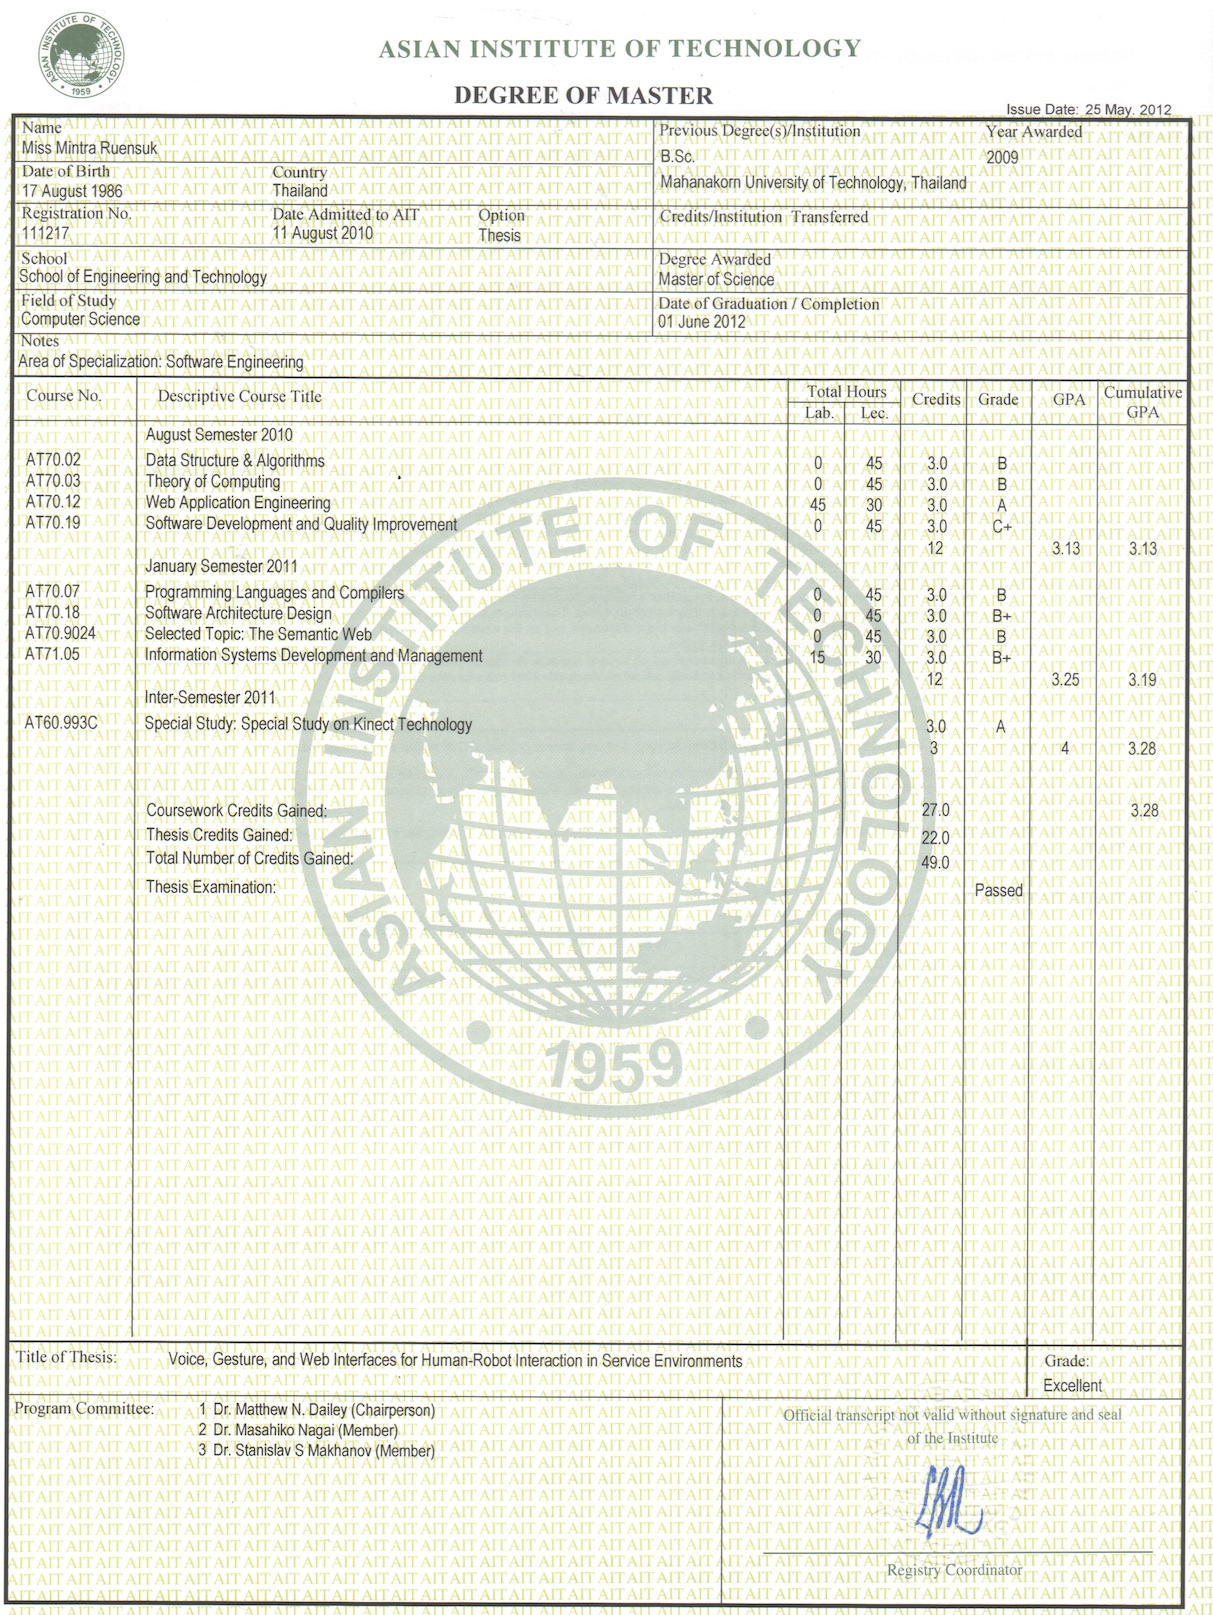
\includegraphics[width=\textwidth]{images/master_1}
\clearpage
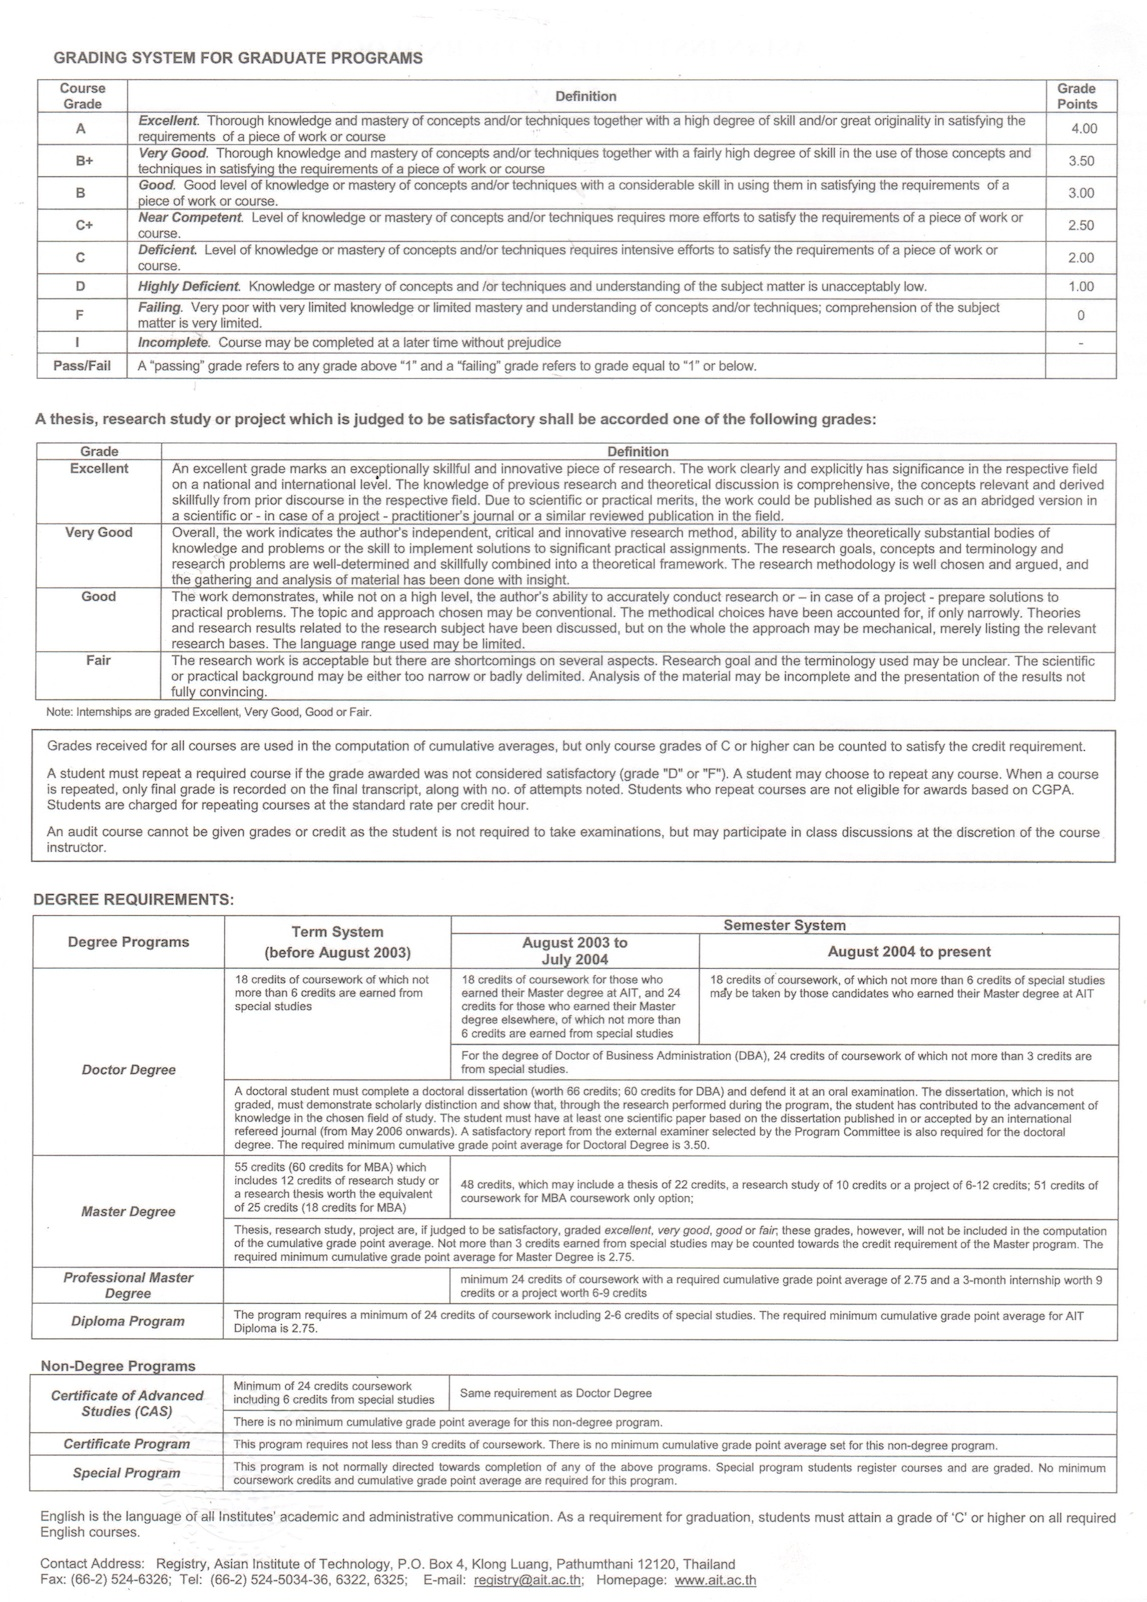
\includegraphics[width=\textwidth]{images/master_2}

\subsection{Bachelor degree}
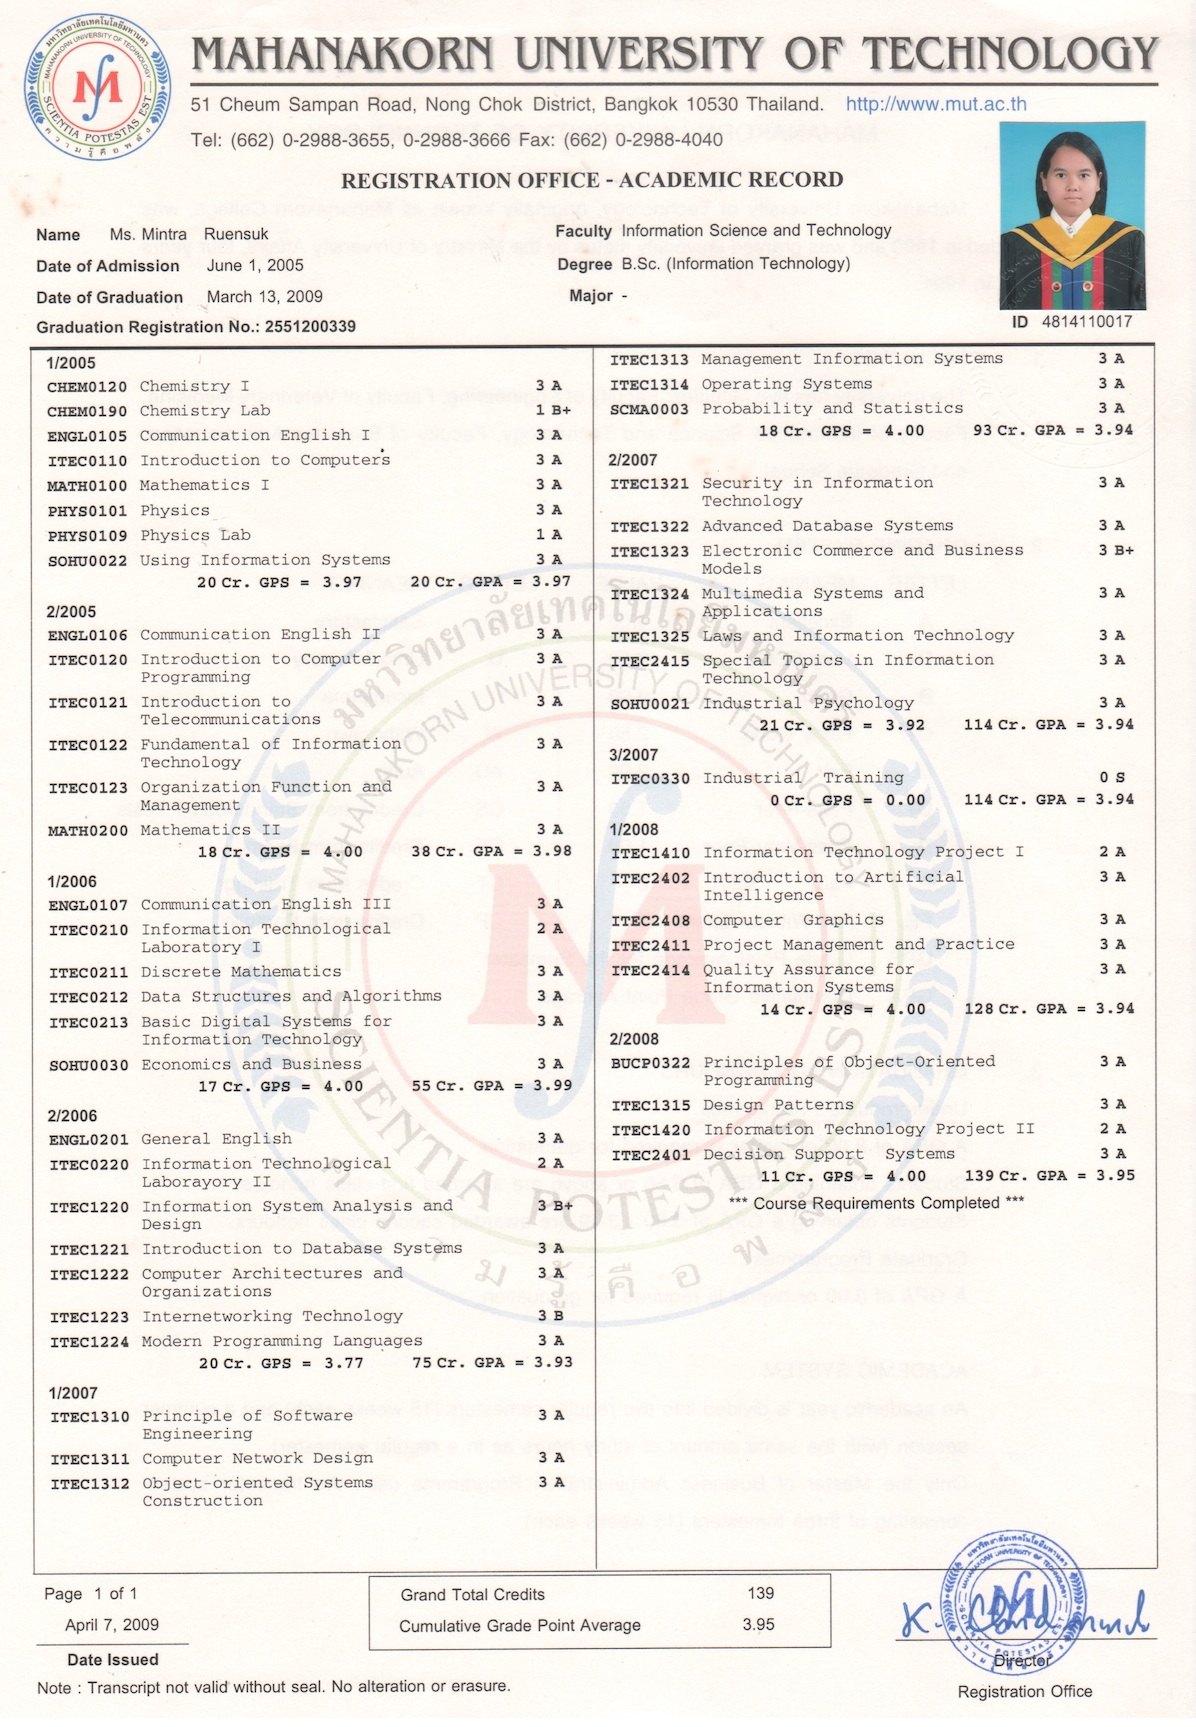
\includegraphics[width=\textwidth]{images/bachelor_1}
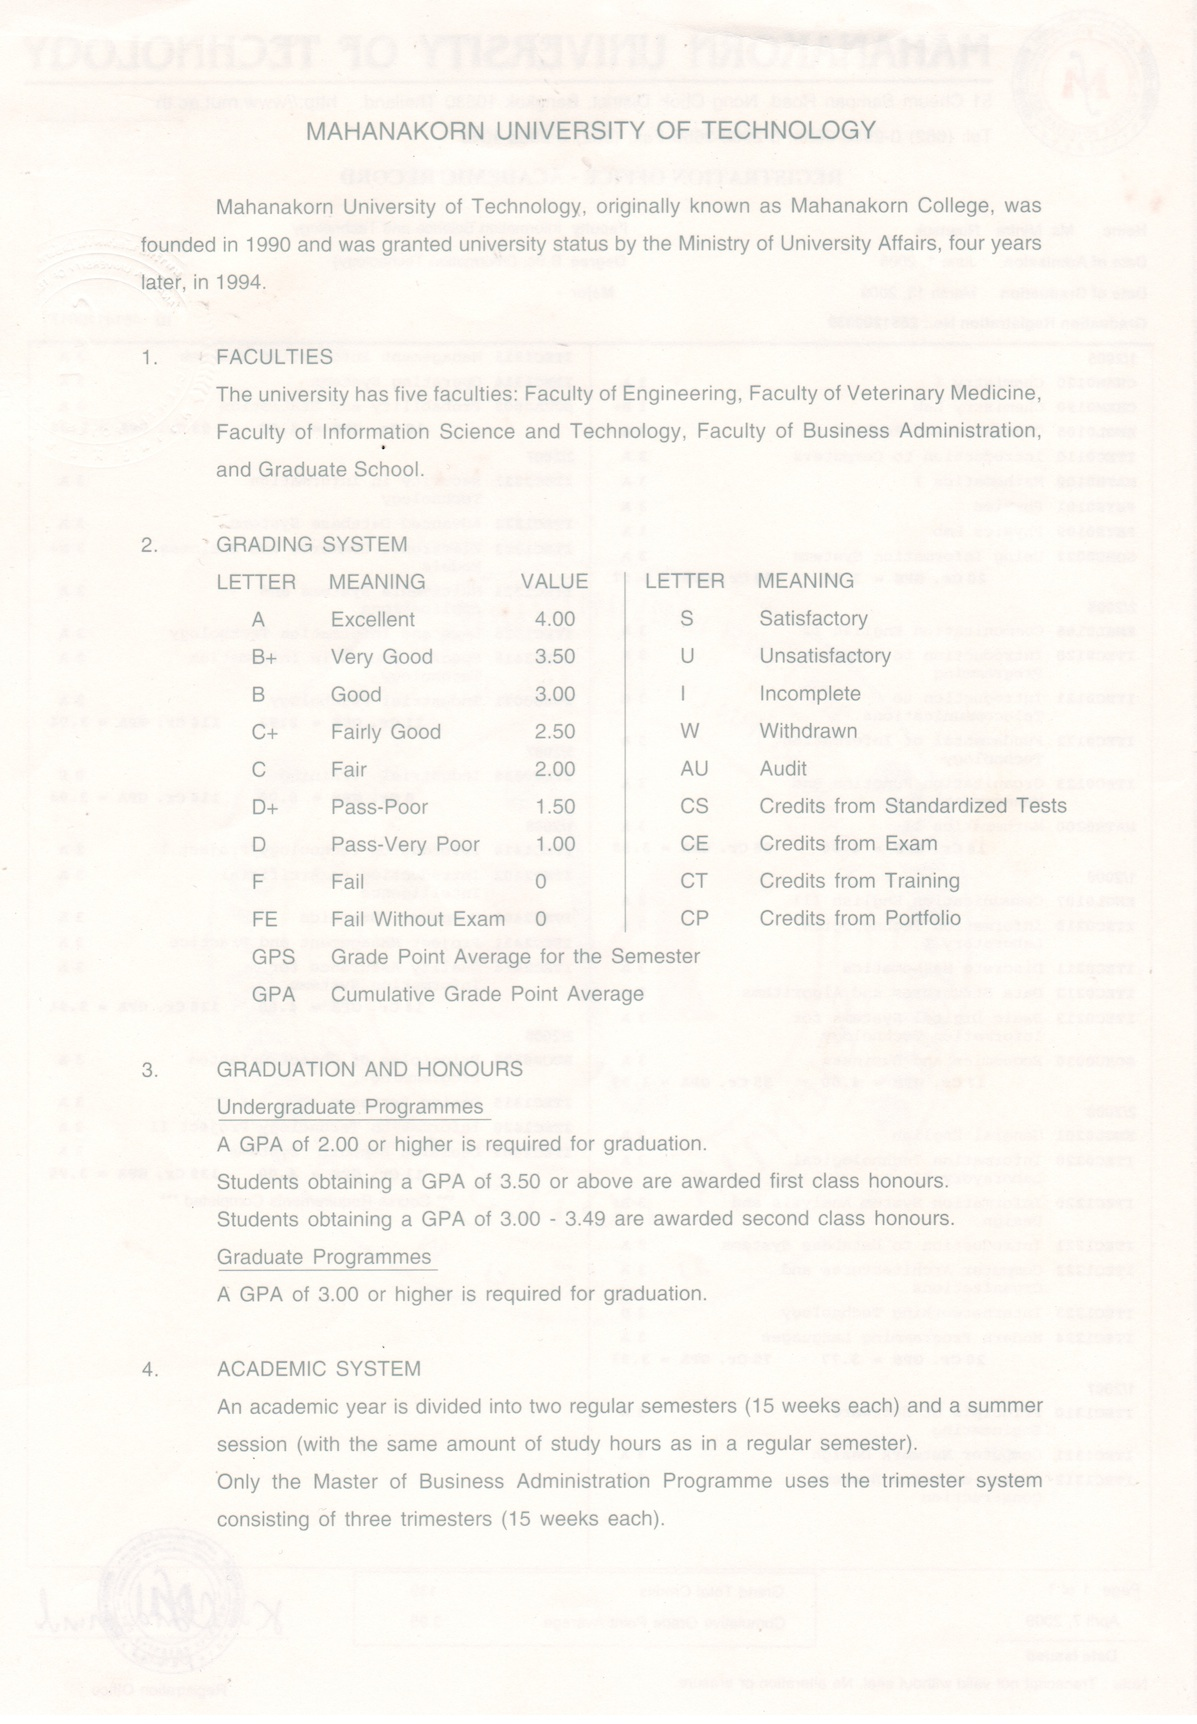
\includegraphics[width=\textwidth]{images/bachelor_2}

\section{Expected start date}
September 1st, 2014
\section{Funding - Do you require funding?}
Yes, I do.

% Publications from a BibTeX file without multibib
%  for numerical labels: \renewcommand{\bibliographyitemlabel}{\@biblabel{\arabic{enumiv}}}% CONSIDER MERGING WITH PREAMBLE PART
%  to redefine the heading string ("Publications"): \renewcommand{\refname}{Articles}
\nocite{*}
\bibliographystyle{plain}
\bibliography{publications}                        % 'publications' is the name of a BibTeX file

% Publications from a BibTeX file using the multibib package
%\section{Publications}
%\nocitebook{book1,book2}
%\bibliographystylebook{plain}
%\bibliographybook{publications}                   % 'publications' is the name of a BibTeX file
%\nocitemisc{misc1,misc2,misc3}
%\bibliographystylemisc{plain}
%\bibliographymisc{publications}                   % 'publications' is the name of a BibTeX file


%\clearpage\end{CJK*}                              % if you are typesetting your resume in Chinese using CJK; the \clearpage is required for fancyhdr to work correctly with CJK, though it kills the page numbering by making \lastpage undefined
\end{document}


%% end of file `template.tex'.
